\documentclass[11pt, a4paper]{article}
\usepackage[T1]{fontenc} 
\usepackage[utf8]{inputenc}
\usepackage[czech]{babel}
\usepackage{hyperref}
\usepackage[left=2cm, top=3cm, text={17cm, 24cm}]{geometry}
\usepackage{graphicx}
\usepackage{titlesec}
\usepackage{enumitem}
\usepackage{times}
\usepackage{float}
\usepackage{minted}

\urlstyle{same}

\begin{document}

\begin{titlepage}
    \begin{center}
        
        \null
        
        \vspace{5cm}
        
        
\includegraphics[scale=0.1,keepaspectratio]{img/logo_cz.png}
        
        \vspace{3cm}
       
        {\textbf{\Huge Projektová dokumentace}}
        
        \vspace{0.5cm}
        
        {\textbf{\LARGE ISA}}
        
        \vspace{0.5cm}
        
        {\LARGE Přenos souboru skrz skrytý kanál}
        
        \vspace{5cm}
        
         \vfill
    \end{center}
    {\LARGE Karel Norek, xnorek01 \hfill \today}


\end{titlepage}

\large
\pagenumbering{Roman}
\tableofcontents
\clearpage

\pagenumbering{arabic}
\setcounter{page}{1}

\section{Úvod do problematiky}
Cílem tohoto projektu je přenos souboru přes skrytý kanál. 

Pro přenos dat přes síť se požívají pakety. Paket je blok dat maximální velikosti standartně 1500 bytů. Každý paket má v sobě určité hlavičky, které znázorňují, které data paket přenáší, a k čemu slouží. Druhy paketů se rozlišují podle protokolů, které paket přenáší. Jeden z protkolů je například ICMP. 

Dalšími druhy jsou: TCP, ARP, UDP atd.. Jedno ze základních rozdělení paketů je rozdělení na IPv4 nebo IPv6. 

V tomto projektu budeme jako skrytý kanál používat ICMP paket. Aby byl přenos bezpečný, posílané data budeme šifrovat. Na šifrování použijeme šifru \emph{AES}.

\subsection{ICMP}
ICMP neboli Internet Control Message Protocol je protokol, který primárně slouží pro oznámení chyb a diagnostiku sítě. Většinou se používá ke kontrole, jestli se data dostanou na požadovanou adresu v nějakém rozumném čase. Je to jeden z nejdůležitějších protokolů pro hlášení chyb a testování.

Nejjednodušší způsob, jak generovat ICMP pakety, je například pomocí příkazu \textbf{ping}. 
ICMP pakety se dají zneužít. Například ICMP flood attack nebo ping of death. Pro naše účely ICMP paket zneužijeme k posílání dat skrze něj.

\subsection{AES}
Advanced Encryption Standard je bloková šifra, která šifruje 128 bitů dat pomocí šifrovacího klíče. Šifrovací klíč může mít velikost 128, 192, a nebo 256 bitů. 

Algoritmus provede několik transformací dat v iteracích. Čím větši velikost klíče, tím více iterací jednotlivých transformací šifra potřebuje. 

První transformací je substituce dat pomocí substituční tabulky. Druhá a třetí transformace míchají data. Poslední transformace využivá části šifrovacího klíče na šifrování jednotlivých sloupců dat. 


\section{Popis programu}
Program slouží k posílání šifrovaných souborů přes skrytý kanál. Je k tomu použit ICMP paket, do kterého jsou vložena potřebná data k rozšifrování souboru. Program slouží zaroveň jako klient, tak i jako server, záleží pouze na tom, jakým způsobem je spuštěn. Ke spuštění programu je potřeba mít root práva. To ve většině případů znamená pouštět program přes příkaz \textbf{sudo}.


\section{Implementace}
Projekt je implementován v jazyce C++. Celá implementace je uložena  v souboru \textbf{secret.cpp}.
Nejdříve je nutné přeložit pomocí příkazu \textbf{make} a poté je možné program \textbf{secret} použít. 

Program se skládá ze dvou hlavnách částí: klient a server. Při spuštění programu lze specifikovat, která část se má spustit pomocí argumentu \textbf{-l}. Pokud je tento argument zadán, program funguje jako server, pokud ne, tak jako klient.

\subsection{Parsování argumentů}
Program začne parsováním argumentů. Pro tento účel existuje třída ArgumentParser, která má atributy pro každý možný argument programu. 
Pro parsování se používá funkce getopt z knihovny \emph{getopt.h}.

\begin{flushleft}
Mezi možné argumenty patří:
\end{flushleft}

 \begin{itemize}
      \item -r file : Pokud je spuštěn klient, argument je povinný a specifikuje, který soubor se má poslat. Tento argument u serveru nemá vliv.
      \item -s IP : Pokud je spuštěn klient, argument je povinný a specifikuje, na kterou adresu se má soubor poslat. Tento argument u serveru také nemá žádný vliv.
      \item -l : Pokud je zadán argument, spustí se program jako server, pokud ne, spustí se jako klient.

\end{itemize}

\subsection{Šifrování}
Program používá \emph{AES} šifrování. Jako klíč je použit \emph{xnorek01}. Pro nastavení klíčů jsou použity funkce \textbf{AES\_set\_encrypt\_key} a \textbf{AES\_set\_decrypt\_key}. Na zašifrování se používá funkce \textbf{AES\_encrypt}, na rozšifrování obdobně \textbf{AES\_decrypt}. Tyto funkce šifrují 16 bytů dat. Pokud není velikost dat 16 bytů, tak funkce sama zbytek bytů doplní. 


\begin{minted}{c++}
char *encrypt(char *data, int length){
    unsigned char *output = (unsigned char *)calloc(length + 
                                    COMPLEMENT(length), sizeof(char));
    if (output == nullptr) {
        std::cerr << "Allocation failed" << std::endl;
        return nullptr;
    }
    for (int shift = 0; shift < length; shift += AES_BLOCK_SIZE) {
        AES_encrypt((unsigned char*)(data + shift), (output + 
                                        shift), &key_e);
    }
    return (char *)output;
}
\end{minted}


Uvedený kód výše je funkce pro zašifrování textu. Nejdříve si musíme alokovat dostatek místa pro výsledek šifrování. Na to je použita funkce calloc. Velikost je určena parametrem funkce length, ke kterému je přičten doplněk, aby velikost byla dělitelná 16. Na doplněk je použito makro \emph{COMPLEMENT}.


\begin{minted}{c++}
#define COMPLEMENT(x) (AES_BLOCK_SIZE - (x % AES_BLOCK_SIZE))
\end{minted}


Poté funkce iteruje skrze pole zadané parametrem data a každých 16 bytů zašifruje a uloží do pole output. Po zašifrování funkce vrací pole output s plně zašifrovanými daty.

Funkce na rozšifrování dat decrypt funguje analogicky, pouze se volá funkce \textbf{AES\_decrypt} místo funkce \textbf{AES\_encrypt}.

\subsection{Struktura pro vlastní protokol}
V posílaných paketech je uložena vlastní struktura s názvem secrethdr, díky které je možné jednoduše identifikovat jestli se jedná o paket poslaný klientem a také umožňuje snadný přístup k datům.

\vspace{0.5cm}

\begin{minted}{c++}
struct secrethdr{
    const char id[AES_BLOCK_SIZE];
    int type;
    int length = 0;
    char data[MAX_DATA_LEN];
};
\end{minted}


Proměnná id je identifikátor paketu. V programu je tento identifikátor zvolen jako slovo \emph{Secretga}. Pomocí tohoto identifikátoru server zjistí, jestli to je paket od klienta, a podle toho pokračuje dál.

Proměnná type je typ paketu. Existují 3 typy. Typ 1 je úvodní paket, který místo dat obsahuje název souboru. Typ 2 je typ, díky kterému server ví, že má přenesená data do souboru. Poslední typ 3 se používá na kontrolu, jestli byly odchyceny všechny odeslané pakety.

Proměnná length udává jakou velikost mají poslaná data. Tato proměnná je nutná, abychom po rozšifrování dat věděli, jakou velikost zapsat do souboru a nevypisovali nechtěná data přidělená funkcí AES\_decrypt. Nechtěná data vzniknou tehdy, když velikost dat není dělitelný 16.

Pole data uschovává posílané data. V úvodním paketu je zde obsažen název souboru, a poté jsou zde uložena zašifrovaná data souboru.

\subsection{Klient}
Klient začíná ve funkci client. Zde za pomocí struktury \emph{addrinfo}, a s ní související funkce \textbf{getaddrinfo}, dostaneme základní informace, abychom mohli vytvořit soket. Jedna z takových informací je například typ protokolu (IPv4 nebo IPv6). Poté se pomocí funkce vytvoří soket. Jakmile je soket vytvořen, zavolá se funkce \textbf{send\_file}, která zařídí posílání souboru.

Ve funkci \textbf{send\_file} se nejdříve zašifruje název souboru a identifikátor paketu. Poté se vytvoří potřebné hlavičky paketů. V tomto případě to je ICMP hlavička a již zmiňovaná struktura secrethdr.
Jako IMCP kód se používá \emph{ICMP\_ECHO}. Nejprve se vytvoří první paket, kde se místo dat přenese název souboru, aby server vědel, jaký soubor vytvořit, popřípadě přepsat. Pro paket se vypočítá checksum z funkce poskytnuté v souborech k předmětu ISA. Jakmile je paket připraven, pošle se přes příkaz sendto na danou IP.

Následuje čtení souboru. Čte se po částech velkých 1024 bytů, aby se data mohla vlézt do standartní velikosti paketu. Načtená data se zašifrují a uloží do atributu data struktury \emph{secrethdr}. Znovu se vypočítá checksum a paket je poslán. Tento proces se v iteracích opakuje dokud se nenačtou všechna data ze souboru. Během čtení se také počítá celková délka. Tato délka je využita v konečném paketu pro kontrolu na straně serveru, jestli se neztratily pakety. Po poslání souboru se tedy pošle poslední paket bez data, sloužící pouze pro kontrolu. Tímto klient končí.

Během posílání dat je použita funkce \textbf{poll} z knihovny \emph{poll.h}, aby se pakety odesílaly pouze tehdy, jakmile jsou připravené.
\subsection{Server}

Pokud je program spuštěn jako server, zavolá se funkce server. Zde se chytají pakety. Pro chytání paketů je využita knihovna \textbf{pcap/pcap.h}. Jako filter je použit \emph{icmp or icmpv6}, který chytá pouze ICMP pakety. Rozhraní, na kterém se pakety zachycují, se nazývá \emph{any}.

Následuje samotné chytaní paketů. Na to se zde používá upravený kód z \cite{Tcpdump}. Změnou je použití \textbf{pcap\_loop} místo \textbf{pcap\_next}. Pokud nenaskytne chyba během otevíraní rozhraní, případně nastavovaní filtru, volá se funkce \textbf{pcal\_loop}, která když zachytí packet, volá callback funkci \textbf{gotPacket}.

Ve funkci \textbf{got\_packet} se nejdříve pomocí struktury \emph{sll\_header} (Linux cooked capture) zjistí typ protokolu a podle zjištěného protokolu se přetypuje paket na strukturu secrethdr.

Nyní se rozšifruje položka na místě, kde by paket poslaný klientem měl identifikátor. Pokud se identifikátor shoduje s globální proměnnou udávající zvolený identifikátor, pokračuje se dál. V opačném případě se nejedná o paket poslaný klientem a funkce končí.

Pokud se jedná o požadovaný paket, následuje rozdělení podle typu paketu (atribut type struktury \emph{secrethdr}). Jedná-li se o typ \emph{START}, rozšifruje se název souboru a vytvoří se, případně přepíše, pokud již soubor existoval. Je-li to typ \emph{TRANSFER}, data se rozšifrují a ukládaji se do vektoru \emph{buffer}. Ten, pokud dosáhne velikosti 5MiB, je vypsán do souboru a vynulován. Tento buffer je použit z důvodu, aby nedocházelo k zahlcení programu díky I/O operacím. Jedná-li se o poslední typ \emph{END}, vypíše se zbytek bufferu a provede se kontrola, jestli nebyl ztracen nějaký paket. Poté klient vypíše hlášku "File transfered", aby uživatel dostal zpětnou vazbu.

Jakmile funkce \textbf{got\_paket} skončí, server se vrací do \textbf{pcap\_loop}, kde čeká na další paket.

\section{Návod na použití}
Pro detailnější návod lze využít soubor \textbf{secret.1}, který slouží jako manuálová stránka. Manuálová stránka lze zobrazit pomocí následujícího příkazu: 

\begin{minted}{bash}
$ man -l secret.1 
\end{minted}

\begin{flushleft}

Spuštění klienta a poslání souboru s názvem file na lokální počítač:
\begin{minted}{bash}
$ sudo ./secret -r test -s 127.0.0.1
$ sudo ./secret -r test -s localhost
\end{minted}

Spuštění serveru:

\begin{minted}{bash}
$ sudo ./secret -l
\end{minted}

\end{flushleft}

\section{Testování}
Testování bylo prováděno ve 2 fázích. První fazí bylo testování na lokálním počítači, kde se posílaly soubory pouze lokálně. Druhá fáze testování spočívala v posílání souborů z virtuálního stroje zpátky na lokální počítač. Textové soubory byly porovnávány pomocí příkazu \textbf{diff} (v obrázcích z testování je proveden výpis pomocí příkazu \textbf{cat} pro porovnání souborů). Obrázky a videa pomocí příkazu \textbf{md5sum}.

\vspace{0.2cm}
\begin{flushleft}
Testované prostředí: Ubuntu 20.04.2 - virtuální stroj, Arch Linux 5.14.15 - lokální počítač
\end{flushleft}

\subsection{1. fáze - Arch Linux}

\begin{flushleft}


\subsubsection{Poslání textového souboru}

\begin{figure}[H]
    \centering
    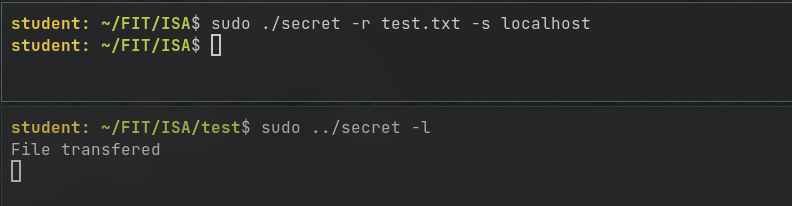
\includegraphics[scale=0.6, keepaspectratio]{img/send_txt.png}
    \label{fig:txt}
 \end{figure}
 
 \begin{figure}[H]
    \centering
    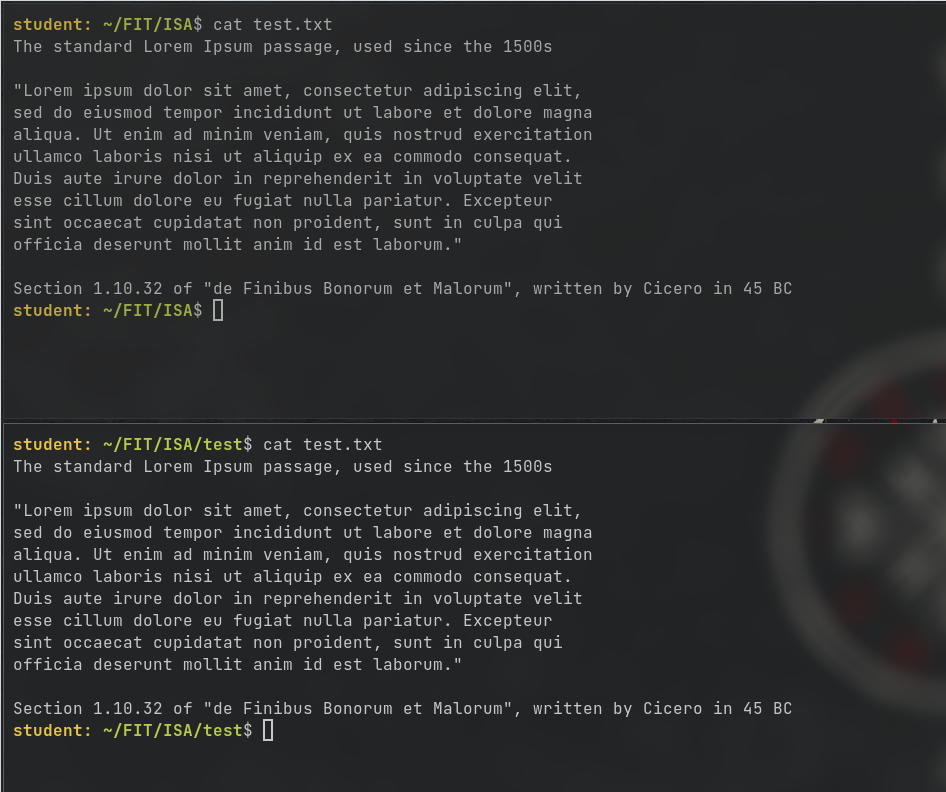
\includegraphics[scale=0.5, keepaspectratio]{img/cmp_txt.png}
    \label{fig:txt}
 \end{figure}



\subsubsection{Poslání již existujícího souboru}

\begin{figure}[H]
    \centering
    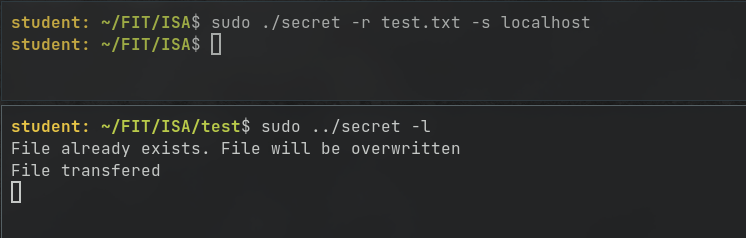
\includegraphics[scale=0.63, keepaspectratio]{img/send_dup_txt.png}
    \label{fig:txt}
 \end{figure}

 
 \begin{figure}[H]
    \centering
    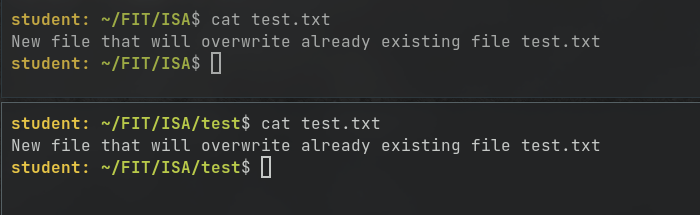
\includegraphics[scale=0.67, keepaspectratio]{img/cmp_txt2.png}
    \label{fig:txt}
 \end{figure}


\subsubsection{Poslání textového souboru, kde soubor má v názvu mezeru}

\begin{figure}[H]
    \centering
    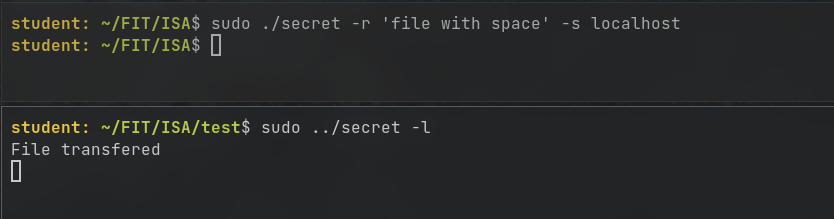
\includegraphics[scale=0.56, keepaspectratio]{img/send_space.png}
    \label{fig:txt}
 \end{figure}
 
 \begin{figure}[H]
    \centering
    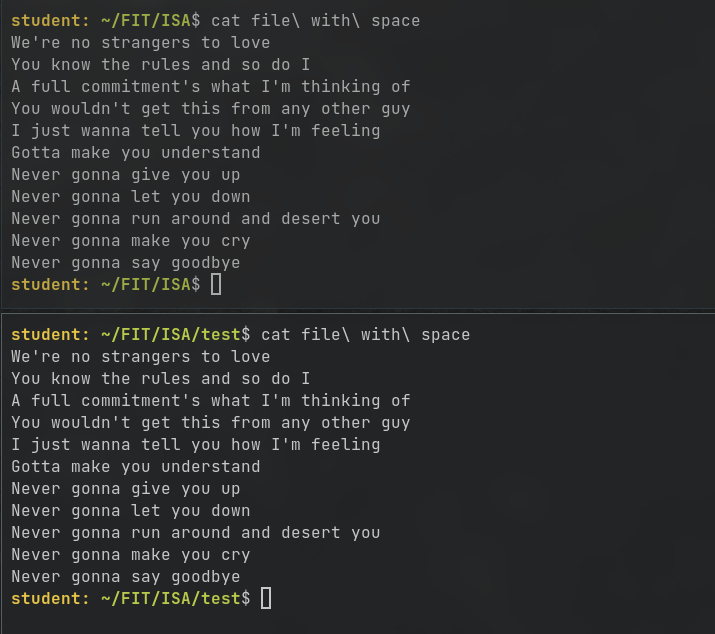
\includegraphics[scale=0.65, keepaspectratio]{img/cmp_space.png}
    \label{fig:txt}
 \end{figure}


\subsubsection{Poslání obrázku}

 \begin{figure}[H]
    \centering
    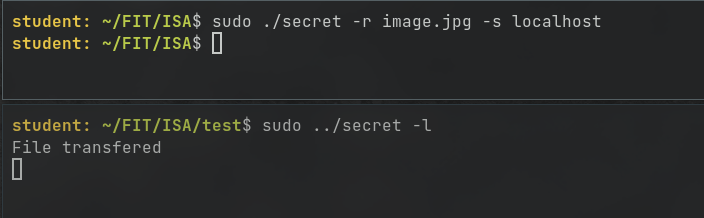
\includegraphics[scale=0.65, keepaspectratio]{img/send_img.png}
    \label{fig:txt}
 \end{figure}
 
  \begin{figure}[H]
    \centering
    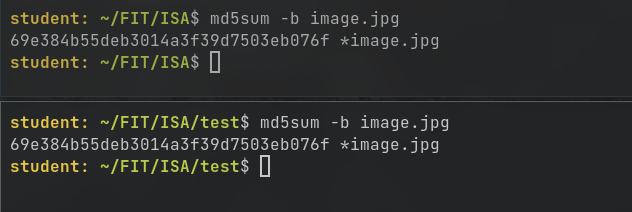
\includegraphics[scale=0.72, keepaspectratio]{img/cmp_img.png}
    \label{fig:txt}
 \end{figure}

\subsubsection{Poslání obrázku většiho než 10MB}

 \begin{figure}[H]
    \centering
    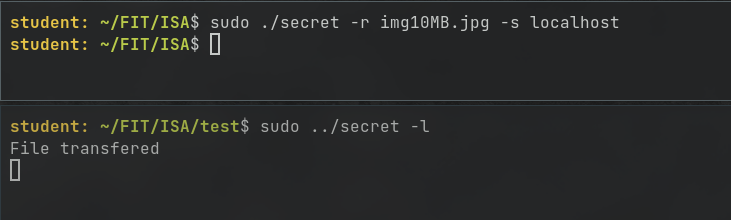
\includegraphics[scale=0.62, keepaspectratio]{img/send_10mb.png}
    \label{fig:txt}
 \end{figure}
 
  \begin{figure}[H]
    \centering
    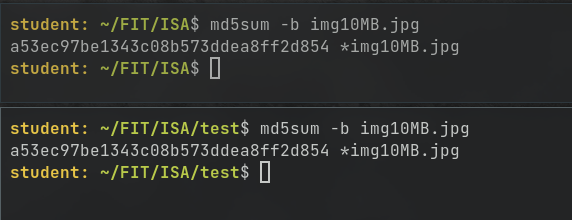
\includegraphics[scale=0.79, keepaspectratio]{img/cmp_10.png}
    \label{fig:txt}
 \end{figure}

\subsubsection{Poslání videa}

 \begin{figure}[H]
    \centering
    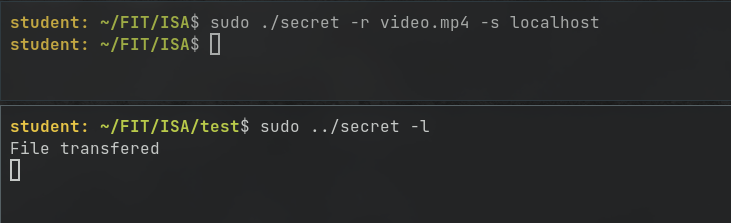
\includegraphics[scale=0.62, keepaspectratio]{img/send_vid.png}
    \label{fig:txt}
 \end{figure}
 
  \begin{figure}[H]
    \centering
    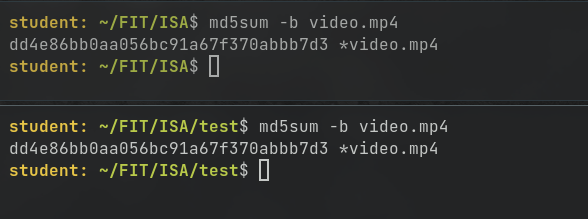
\includegraphics[scale=0.77, keepaspectratio]{img/cmp_vid.png}
    \label{fig:txt}
 \end{figure}


\subsection{2. fáze - Ubuntu na Arch Linux}

\subsubsection{Poslání textového souboru}
\begin{figure}[H]
    \centering
    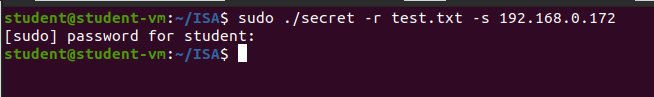
\includegraphics[scale=0.7, keepaspectratio]{img/ub_send_txt1.png}
    \label{fig:txt}
 \end{figure}
 
  \begin{figure}[H]
    \centering
    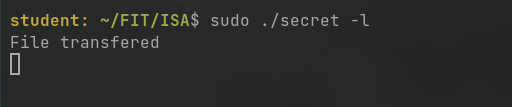
\includegraphics[scale=0.89, keepaspectratio]{img/ub_send_txt2.png}
    \label{fig:txt}
 \end{figure}

\begin{figure}[H]
    \centering
    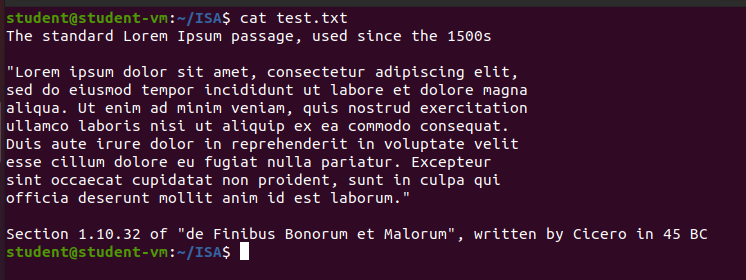
\includegraphics[scale=0.61, keepaspectratio]{img/ub_cmp_txt1.png}
    \label{fig:txt}
 \end{figure}
 
  \begin{figure}[H]
    \centering
    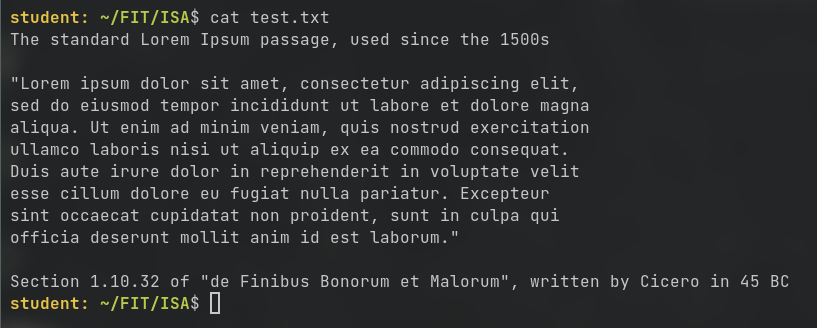
\includegraphics[scale=0.56, keepaspectratio]{img/ub_cmp_txt2.png}
    \label{fig:txt}
 \end{figure}


\subsubsection{Poslání obrázku většiho než 10MB}

\begin{figure}[H]
    \centering
    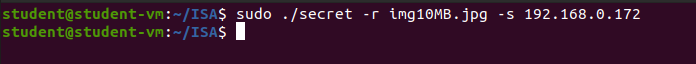
\includegraphics[scale=0.66, keepaspectratio]{img/ub_send_10.png}
    \label{fig:txt}
 \end{figure}
 
  \begin{figure}[H]
    \centering
    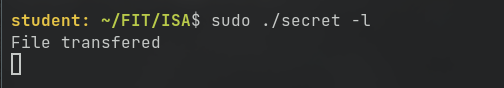
\includegraphics[scale=0.91, keepaspectratio]{img/ub_send_101.png}
    \label{fig:txt}
 \end{figure}
 
 \begin{figure}[H]
    \centering
    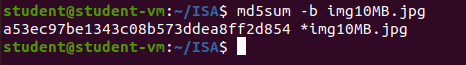
\includegraphics[scale=0.98, keepaspectratio]{img/ub_cmp_10.png}
    \label{fig:txt}
 \end{figure}
 
  \begin{figure}[H]
    \centering
    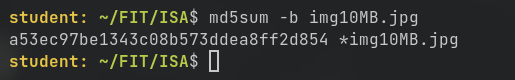
\includegraphics[scale=0.86, keepaspectratio]{img/ub_cmp_101.png}
    \label{fig:txt}
 \end{figure}

\subsubsection{Poslání videa}

\begin{figure}[H]
    \centering
    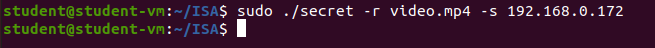
\includegraphics[scale=0.67, keepaspectratio]{img/ub_send_vid.png}
    \label{fig:txt}
 \end{figure}
 
  \begin{figure}[H]
    \centering
    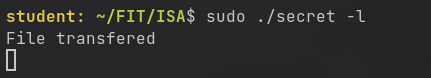
\includegraphics[scale=1.02, keepaspectratio]{img/ub_send_vid1.png}
    \label{fig:txt}
 \end{figure}
 
 \begin{figure}[H]
    \centering
    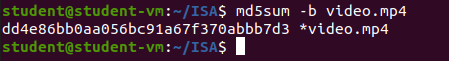
\includegraphics[scale=0.98, keepaspectratio]{img/ub_cmp_vid.png}
    \label{fig:txt}
 \end{figure}
 
  \begin{figure}[H]
    \centering
    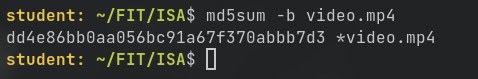
\includegraphics[scale=0.92, keepaspectratio]{img/ub_cmp_vid1.png}
    \label{fig:txt}
 \end{figure}

\end{flushleft}
\section{Závěr}
Při správném postupu klient posílá ICMP pakety, které obsahují zašifrovaný soubor. Správně je i posílá na zadanou IP adresu. Server zvládne ochytávat příchozí pakety, kontrolovat, jsou-li to pakety zaslané klientem, a pokud ano, dešifrovat jejich obsah a zapsat přenášený soubor do lokální složky, kde je server spuštěn.

\newpage

\section{Použité zdroje}
\nocite{*}
\renewcommand{\section}[2]{}
\bibliographystyle{czechiso}
\bibliography{literatura}

    
\end{document}